\documentclass[11pt]{article}
\usepackage{geometry}                % See geometry.pdf to learn the layout options. There are lots.
\geometry{letterpaper}                   % ... or a4paper or a5paper or ... 
\geometry{margin=1in}                   % all margins 1 inch 
%\geometry{landscape}                % Activate for for rotated page geometry
\usepackage[parfill]{parskip}    % Activate to begin paragraphs with an empty line rather than an indent
\usepackage{graphicx}
%\usepackage{amssymb}
\usepackage{latexsym,amsmath,amssymb}  % AMS packages
\usepackage{epstopdf}
\usepackage{longtable}
\DeclareGraphicsRule{.tif}{png}{.png}{`convert #1 `dirname #1`/`basename #1 .tif`.png}

% Chose the sans serif font to be helvetica
\usepackage{helvet}
% Chose that default font is sans serif (instead of roman)
\renewcommand{\familydefault}{\sfdefault}

\usepackage{subfigure}
\usepackage{wrapfig}

% % % % % % % % % % % % % % % % % % % % % % % % % % 
%        This packages are to be able to include Matlab code directly copied from Matlab.
%    (see http://ifatwww.et.uni-magdeburg.de/~stkforum/modules/newbb_plus/viewtopic.php?topic_id=186&forum=65)
%
%       If you want to use BW (black&white) instead of matlab colors, un-comment the part after "Monochrome" below.
\usepackage{listings}		% to have Matlab code in colors
\usepackage{textcomp}		% for the " ' " instead of " � "
\lstdefinelanguage{matlabmod}		% defines a new language, adding keywords:
  {morekeywords={break,case,catch,continue,elseif,else,end,for,function,global,
      if,otherwise,persistent,return,switch,try,while},
   morecomment=[l]\%,
   morestring=[m]',
  }[keywords,comments,strings]%
\usepackage{color}			% to define the colors
% set up listings:
% Color
\lstset{language=matlabmod,
	basicstyle=\small\ttfamily,
	keywordstyle=\color[rgb]{0,0,1},
	upquote=true,	% to have "upright" quotes in the listings ( ' instead of � )
	commentstyle=\color[rgb]{0.133,0.545,0.133},
	stringstyle=\color[rgb]{0.627,0.126,0.941},
	frame=single, framexleftmargin=3mm, xleftmargin=0mm,
	numbersep=0mm, numbers=none, numberstyle=\tiny
%	numbersep=3mm, numbers=left, numberstyle=\tiny
}
% \usepackage{LuxiMono}
%% Monochrome
%\lstset{language=matlabmod,
%	basicstyle=\footnotesize\ttfamily,
%	keywordstyle=\bfseries,
%	commentstyle=\color[rgb]{0.66,0.66,0.66}\itshape,
%	stringstyle=\color[rgb]{0.5,0.5,0.5},
%	frame=single, framexleftmargin=6mm, xleftmargin=6mm,
%	numbersep=3mm, numbers=left, numberstyle=\tiny
%}

%    End of style for being able to include Matlab code directly.
% % % % % % % % % % % % % % % % % % % % % % % % % 

\usepackage{hyperxmp}   % Filling xmp fields in PDF
%%%%%%%%%%%%%%
%%     Hyperref     %%
%%%%%%%%%%%%%%
\usepackage{xr-hyper}
\usepackage{hyperref}
\hypersetup{%
    colorlinks=true,
    bookmarksnumbered=true,
    plainpages=false,
    pdftitle={FMRI Data Quality}, 
    pdfauthor={Pablo Velasco, NYU Center for Brain Imaging},
    pdfcopyright={Copyright (C) 2008-2012, New York University}, 
    pdfsubject={electronic technical report},
    pdfkeywords={FMRI, data quality} 
}



%  %  %  %  %  %  %  %  %  %

\title{FMRI Data Quality}
\author{Pablo Velasco}
\date{Version 1.5 -- Jan 24, 2014}


%  %  %  %  %  %  %  %  %  %

\begin{document}
\maketitle

\tableofcontents
\newpage

\section{Purpose}

This tool examines the quality of functional data.  It checks the spatial and temporal statistics of the voxel intensity in a series of ROIs defined by the user, and generates an \texttt{html} report with the quantitative quality indicators (Signal-to-Noise Ratio, Signal-to-Fluctuation-Noise Ratio and Signal-to-Ghost Ratio; defined below); as well as a spike detection report and plots of the average image intensity time-course for those ROIs.  It also includes a function to correct for the spikes detected in the data.


%%%	%%%	%%%	%%%

\section{Introduction}

Temporal stability during fMRI acquisition is of vital importance because the Blood Oxygenation Level Dependent (BOLD) effects of interest are only a few percent in magnitude.  To accurately measure such small signal changes, an MR system must have intrinsic image time series fluctuation levels much lower than these expected signal changes \cite{Friedman:2006fy}.

This document describes the data analysis protocol suggested by CBI to check for the quality of functional data.  It is designed to be run on functional scans \textbf{before} any data processing (before motion correction, smoothing, etc).  By running it on \textbf{all your data series} you will be able to tell beforehand if your data are not worth being analyzed, saving you precious time.


%%%	%%%	%%%	%%%

\section{Description of the analysis}
\label{sec:description}

The code loops through the repetitions\footnote{You can skip some volumes from the beginning of the run, to allow for signal stabilization.}, reads the data (it works for both NIfTI and DICOM formats) and calculates the spatial mean and standard deviation ---for each repetition--- of the signal in a set of regions of interest (ROIs), some of which are in the object, some in the ghost and some in the background.  The location of the ROIs can be calculated automatically by another function (also provided with the package), based on the image dimensions and phase encoding (PE) direction, and can be modified manually by the user.

After obtaining the temporal series of the spatial means and standard deviations for each ROI, a series of statistical indicators are computed, which will give the user a quantitative index of the data quality:

\begin{itemize}
   \item \textbf{SNR$_0$}: Signal-to-Noise Ratio, from \cite{Weisskoff:1996la}. It takes as ``signal" the average voxel intensity in all the ROIs defined in the object, averaged across time. It takes as ``noise" the standard deviation (across space) of the signal in the ROIs defined in the background, and then averaged across time:
   \begin{equation} \label{eq:SNR_0}
\mathsf{SNR}_0 = \frac{ <\left( <S_\mathsf{object}>_x \right)>_t} {1.53 \times < \left[ std_x \left( S_\mathsf{background} \right) \right] >_t}
   \end{equation}
   The 1.53 factor is used to correct for the fact that we took the absolute value of a complex image with 0 mean.
   
   \item \textbf{SFNR}: Signal-to-Fluctuation-Noise Ratio, from \cite{Friedman:2006fy, Glover-GH:2004dp}.  It takes as ``signal" the same as for the SNR$_0$ above.  It takes as ``fluctuation noise" the (temporal) standard deviation of the (spatial) mean in the same ROIs, after the slow drift (quadratic) has been removed from the temporal series.
   \begin{equation*}
\mathsf{SFNR} = \frac
{ <\left( <S_\mathsf{object}>_x \right)>_t}  {std_t \left(  <S_\mathsf{object}>_x \right)}
   \end{equation*}

   \item \textbf{SGR}: Signal-to-Ghost Ratio, from \cite{Simmons:1999rz}.  It takes as ``signal" the average voxel intensity from an ROI inside the object, and then averaged across time. It takes as ``ghost" the average voxel intensity from an ROI in the ghost, corresponding to the previous ROI in the object (that is, half a field of view away), and then averaged across time:
   \begin{equation*}
\mathsf{SGR} = \frac
{ <\left( <S_\mathsf{object-linked-to-ghost}>_x \right)>_t} { <\left( <S_\mathsf{ghost}>_x \right)>_t}
   \end{equation*}

\end{itemize}

Then, it plots the signal time-courses for each ROI group, in which you can check visually for the quality of your data.  Next, it searches for spikes in the signal intensity in a set of ROIs in the background.  Finally, it writes a \texttt{html} report file which includes some information about the scan, the figures, the statistical indicators and the spike detection results.  If any spikes had been detected during the analysis, this tool saves the repetition numbers and the spiky slices in a file, allowing the user to correct the data with an additional function provided in this tool.

Here we describe in a little more detail each of the functions:


%%%

\subsection{roiCorners.m}
\label{sec:roiCorners.m}

\texttt{roiCorners.m} is a function used to automatically generate the default location of a series of ROIs for the data quality check.  If only the name of the data file is passed, it uses the default name \texttt{rois.txt} to store the ROI locations.  If the ROIs file already exists, it doesn't overwrite it and it just displays the location or the ROIs (see Sec. \ref{sec:displayROIs.m}).

The default locations depend on the the acquisition matrix (\emph{e.g.}, 64 x 64), the number of slices and PE direction (obtained from the data header).  The locations are based on the assumption that the object will be in the middle of the field of view and that there is background in all four edges of the image.  The ROIs are classified into four sections (object, ghost, background and `spikes'). These are the default ROIs (see Fig. \ref{fig:h_roi_loc}):

\begin{figure}[htbp]
   \centering
   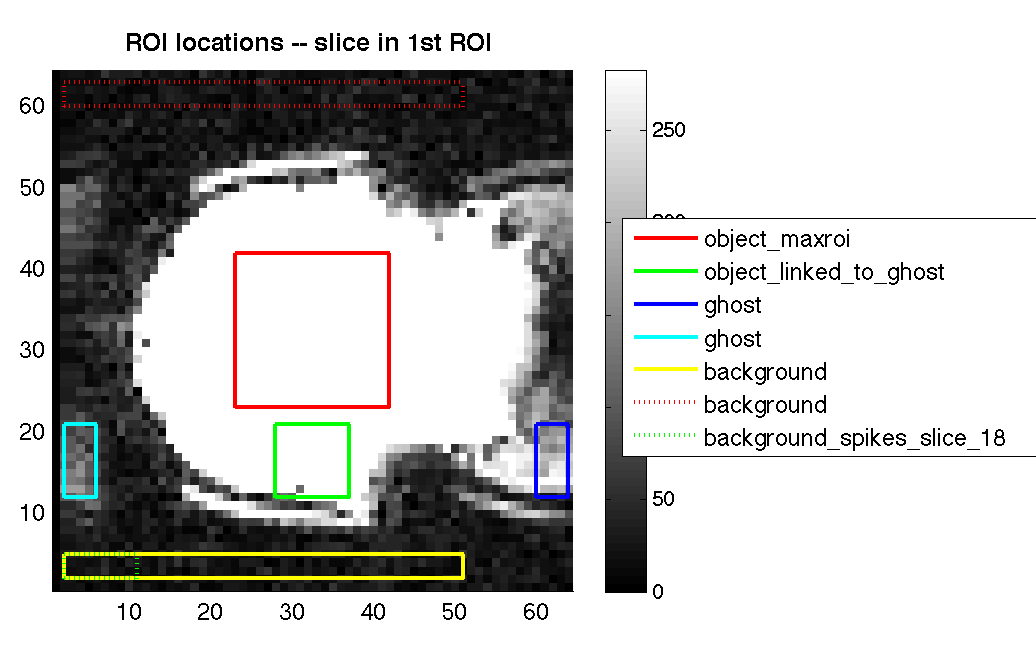
\includegraphics[width=6 in]{images/h_roi_loc.png}
   \caption{Example of the default locations of the ROIs in the central slice from a representative run (the image intensity has been windowed so that the ghost shows up clearly).  This type of plot allows the user to check whether the default placement of the ROIs is correct or if you need to move some of them.}
   \label{fig:h_roi_loc}
\end{figure}

\begin{itemize}
   \item \textbf{Object}:
   \begin{itemize}
      \item 20x20 center of Object (\texttt{object\_maxroi}: red box in the center of the object in Fig. \ref{fig:h_roi_loc}).
      \item 10x10 in Object, the region corresponding to 10x10 ROI in Ghost (that is, Ny/2 away from the ghost in the PE direction). (\texttt{object\_linked\_to\_ghost}: green box right below \texttt{object\_maxroi} in Fig. \ref{fig:h_roi_loc}).
   \end{itemize}
   \item \textbf{Ghost}:
   \begin{itemize}
      \item 1st part on the right (or top, depending on the PE direction) of the central slice, centered at 1/4th of the image along the readout dimension (\texttt{ghost}: navy box at the right of the image in Fig. \ref{fig:h_roi_loc}).
      \item 2nd part on the left (or bottom, depending on the PE direction) of the central slice, centered at 1/4th of the image along the readout dimension (\texttt{ghost}: light blue box at the left of the image in Fig. \ref{fig:h_roi_loc}).
      \end{itemize}
   \item \textbf{Background}:
   \begin{itemize}
      \item 2x50 along one of the edges of the image where there is no ghost, in the central slice (\texttt{background}: yellow box at the bottom of the image in Fig. \ref{fig:h_roi_loc}).
      \item 2x50 at the other edge of the image where there is no ghost, in the central slice  (\texttt{background}: red dotted box at the top of the image in Fig. \ref{fig:h_roi_loc}).
      \end{itemize}
   \item \textbf{Spikes}:
   \begin{itemize}
      \item in every slice, a small (5x10) ROI in the background, to detect spikes  (For the central slice:\texttt{background\_spikes\_slice\_18}: green dotted box at the bottom left of the image in Fig. \ref{fig:h_roi_loc}).
   \end{itemize}
\end{itemize}

Since \textbf{it is very important that you check that the ROIs are in the correct locations}, after the ROIs are saved into a text file, \texttt{roiCorners} calls the function \texttt{displayROIs} (Section \ref{sec:displayROIs.m}) to display them in a figure, like Fig. \ref{fig:h_roi_loc}.

If you need to modify the default location of any of the ROIs, open the file with a text editor.  You will see the different ROIs organized by region, and the entry for each one is preceded by a label and a short description of the ROI, followed by a line with the (\emph{i},\emph{j},\emph{k}) indices of one of the corners of the ROI, and in, the next line, the coordinates of the opposite corner.  Note that the \emph{i},\emph{j},\emph{k} indices start counting from 1, not from 0.

Here is a sample of the first few lines of a ROI file:

\begin{lstlisting}
=== OBJECT ===

OBJECT_MAXROI: 20x20 center of Object
23,23,18
42,42,18

OBJECT_linked_to_Ghost: 10x10 in Object - region corresponding to 10x10 ROI in Ghost
12,28,18
21,37,18


=== GHOST ===

GHOST: 10x10 in Ghost - 1st part: top of slice
12,60,18
21,64,18

...
\end{lstlisting}


%%%

\subsection{importROIs.m}
\label{sec:importROIs.m}

\texttt{importROIs.m} is a function to read the ROI corners from a ROI file.  It loops through all the lines in the file and stores the information in four structure arrays (\texttt{object}, \texttt{ghost}, \texttt{background} and \texttt{spikes}); with each of the elements of the arrays containing the following fields:

\begin{itemize}
   \item \texttt{name}: name of the ROI
   \item \texttt{type}: the type of the ROI: \texttt{object}, \texttt{ghost}, \texttt{background} or \texttt{spikes}
   \item \texttt{corner1}: indices (\emph{i},\emph{j},\emph{k}) of the first ROI corner.
   \item \texttt{corner2}: indices (\emph{i},\emph{j},\emph{k}) of the second (opposite) ROI corner.
   \item \texttt{nvox}: total number of voxels in this ROI
   \item \texttt{meants}: time-series of the mean voxel intensity across the ROI.
   \item \texttt{stdts}: time-series of the standard deviation of the voxel intensities across the ROI.
\end{itemize}

Since \texttt{importROIs} only reads the information contained in the ROI file, the last two fields (\texttt{meants} and \texttt{stdts}) are returned empty.  They will be used by \texttt{checkdataquality.m} (Section \ref{sec:checkdataquality.m}) to store the corresponding ROI statistics for each time-point.


%%%

\subsection{displayROIs.m}
\label{sec:displayROIs.m}

\texttt{displayROIs.m} is a function used to display the location of some of the most relevant ROIs with respect to the image.

It first calls \texttt{importROIs.m} (Section \ref{sec:importROIs.m}) to read the ROIs locations, and then gets the first volume of data in the image file to generate the image.  With these, it selects the the slice corresponding to the first corner of the first ROI in the ROIs file.  It creates a figure showing that slice as well as colored rectangles showing all the ROIs present in that specific slice.  An example of such an image is Fig. \ref{fig:h_roi_loc}.


%%%

\subsection{checkdataquality.m}
\label{sec:checkdataquality.m}

\texttt{checkdataquality.m} is the function which does the statistical computations and generates the images.

As with \texttt{roiCorners.m}, the first thing \texttt{checkdataquality} does is to read the file header, to obtain the acquisition matrix (\emph{e.g.}, 64 x 64), the number of slices and repetitions, and the PE direction.  If the \texttt{*-header.txt} file created at  extraction from CBI-webdb is present in the same folder as the data file, \texttt{checkdataquality} reads the date the data were collected as well as the coil that was used.

Then, \texttt{checkdataquality} calls \texttt{importROIs.m} to get the location of the ROIs.  Once the function knows where the ROIs are, it loops through the repetitions (a.k.a. volumes, measurements or time-points), reading one volume at a time and, for each of the ROIs, it calculates the mean voxel intensity (and the standard deviation) across the ROI.  It also calculates the mean voxel intensity of all ROIs in each of the three regions: \texttt{object}, \texttt{ghost} and \texttt{background}.  The user can specify how many time-points to exclude from the beginning of the run (the default is zero).

When all the repetitions have been read, it calculates the 3 statistical indicators described in Sec. \ref{sec:description} and plots 3 graphs, with the time courses of the average voxel intensity in the ROIs in the \texttt{object}, \texttt{background} and \texttt{ghost}, respectively.  In them, you can observe the size of the fluctuations, and the intensity in the background, compared to the image intensity.

Finally, \texttt{checkdataquality} runs a ``\emph{search for spikes}".  In it, for each of the ROIs in the \texttt{spikes} section of the ROI file, the function does a search for peaks in the intensity.  A time point is tagged as a `peak' when the signal is bigger than `threshold' standard deviations above the mean (across time).  The threshold is set to 10, which seems to be very effective at catching spikes, without giving many false positives.  Internally, it saves the spike candidates in a structure called \texttt{peaks}, with fields:

\begin{itemize}
   \item \texttt{ts}: timepoints where a spike was detected (for that ROI);
   \item \texttt{nspk}: number of spikes (again, for that ROI);
   \item \texttt{slices}: slices included in that ROI;
   \item \texttt{name}: name of the ROI where those spikes were found.
\end{itemize}

The spike detection part of \texttt{checkdataquality} also plots the time courses of the mean signal for each of the \texttt{spikes} ROI.  The data would be noisy, but normally without any big peak (for example, see Fig. \ref{fig:h_spikes_normal}).  An example of a time-course with ``big peaks" is given in Fig. \ref{fig:h_spikes_spiky}.  In the plot you can evaluate visually how big the detected peaks are.  If the "spike detection" part picked up any spike candidates, the script will also generate a graph for each of the candidates in which it will show the image of the corresponding slice for the bad timepoint (in the middle) and the adjacent timepoints both before and after the bad timepoint (Fig. \ref{fig:h_spiky_slices_1}).

\begin{figure}[htbp]
   \centering
   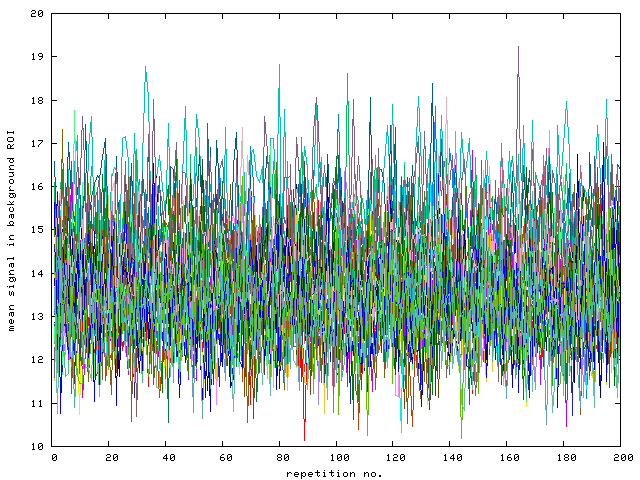
\includegraphics[width=5 in]{images/h_spikes_normal.png}
   \caption{Example of the time-course in the \texttt{spikes} ROIs for a normal run.  Note how the noise fluctuation size is very constant across time and the baseline is similar for all ROIs.}
   \label{fig:h_spikes_normal}
\end{figure}

\begin{figure}[htbp]
   \centering
   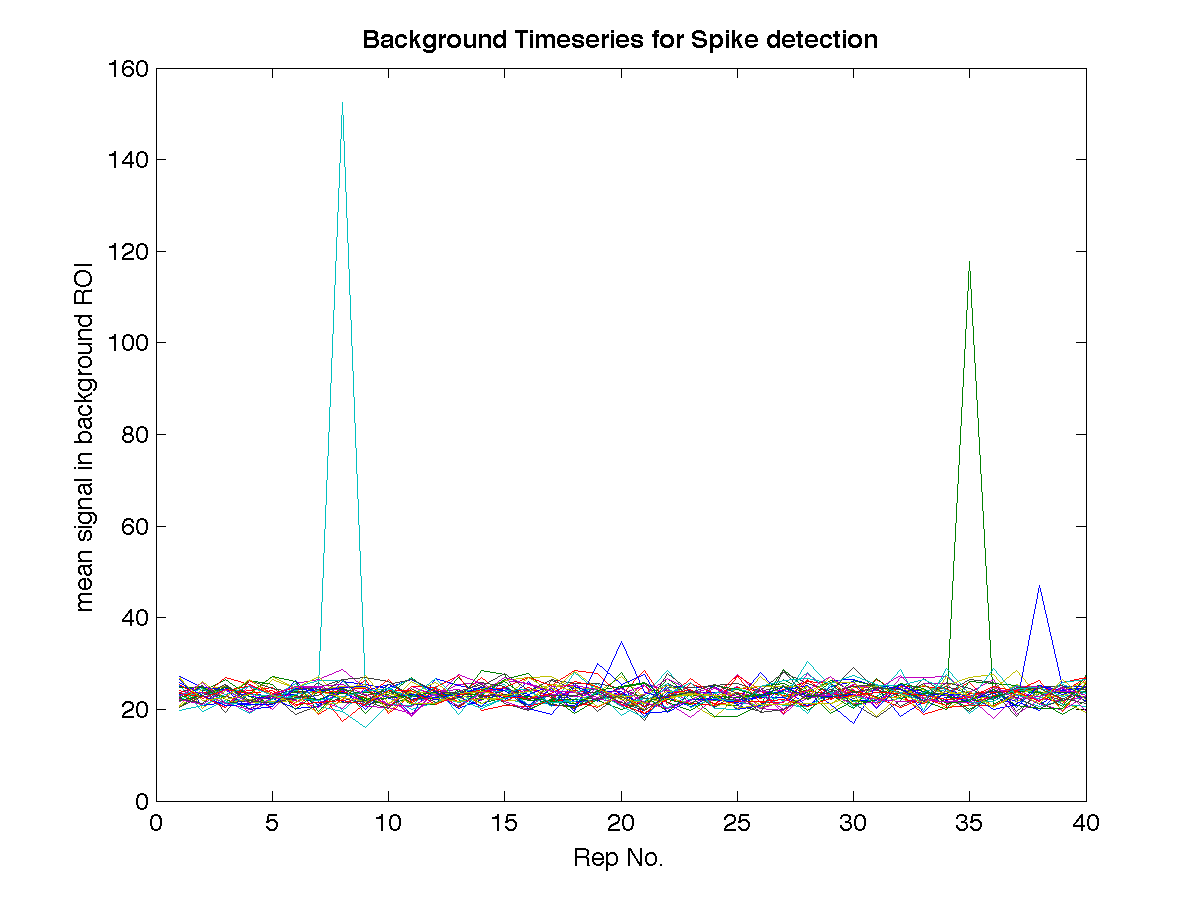
\includegraphics[trim = .5in .2in .4in .18in, clip,width=5 in]{images/h_spikes_spiky.png}
   \caption{Example of the time-course in the \texttt{spikes} ROIs for a ``spiky" run.  There are three peaks standing up above the baseline level.}
   \label{fig:h_spikes_spiky}
\end{figure}


\begin{figure}[htbp]
   \centering
   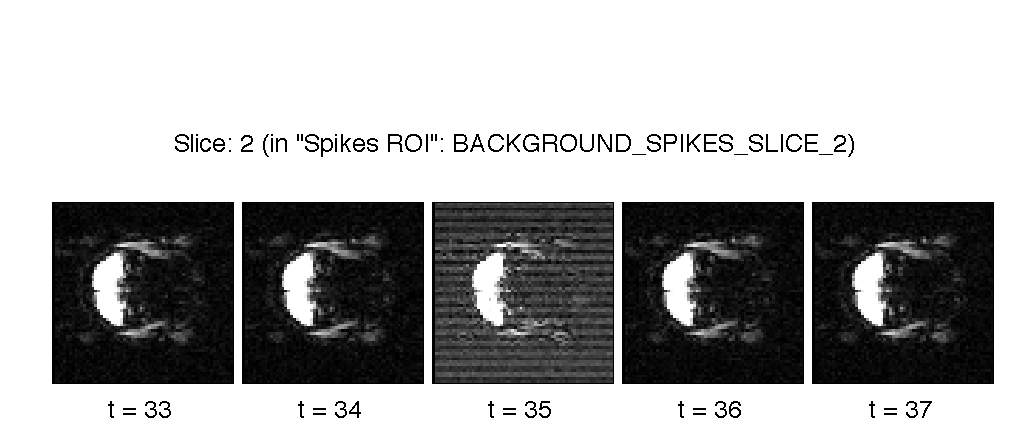
\includegraphics[trim = .35in .1in .25in .8in, clip,width=5 in]{images/h_spiky_slices_1.png}
   \caption{Images of the slice showing a peak in the intensity at time-point 35 in Fig. \ref{fig:h_spikes_spiky}, and the same slice for the two timepoints before and after.  Note the corduroy pattern across the image, typical of spikes.}
   \label{fig:h_spiky_slices_1}
\end{figure}


%%%

\subsection{dataQReport.m}
\label{sec:dataQReport.m}

\texttt{dataQReport.m} is the function that generates an \texttt{html} report of the results from \texttt{checkdataquality}.  The function creates a folder (inside the same folder as the data being checked) called \texttt{qReport\_datafName}, where \texttt{datafName} is the name of the data file being analyzed (with no extension).

The first step is to run \texttt{checkdataquality} and to save the images created (as \texttt{png} files).  Then, \texttt{dataQReport} writes out the \texttt{html} file, line by line, which includes:

\begin{itemize}
   \item The coil used to collect the data.
   \item The date of the study.
   \item The plot with the ROI locations (see Section \ref{sec:displayROIs.m}).
   \item The SNR ``indicators".
   \item The time-series plots for the intensity in the three ROI sections: \texttt{object}, \texttt{background} and \texttt{ghost}.
   \item The results of the ``spike detection": Total number of potential spikes, and the time-point and ROI where they occurred; the time-series plot of the intensity in all the \texttt{spikes} ROIs and, in the case any possible spikes are detected, the plot of the slice and time-point where they were detected (and the 2 previous and posterior time-points for that same slice, for comparison).
\end{itemize}

Finally, \texttt{dataQReport} copies the ROI file used to generate the report in the same folder containing the report.  The idea is that if the user thinks the CBI staff should take a look at the results, he/she can zip the whole folder that was created and email to the corresponding person.  Then, the zip file will contain all the information the CBI staff would need to analyze the data.

\texttt{dataQReport.m} returns a structure with the following fields:

\begin{itemize}
   \item \texttt{snr0}
   \item \texttt{sfnr}
   \item \texttt{sgr}
   \item \texttt{sDate}: scan date
   \item \texttt{coil}: coil used for the scan
   \item \texttt{peaks}: structure containing the information about spikes in the data (see \ref{sec:checkdataquality.m}).
\end{itemize}


%%%

\subsection{correcting\_spikes.m}
\label{sec:correcting_spikes.m}

A new version (v 2.0) of \texttt{correcting\_spikes.m} has been included with the distribution.  This function corrects bad timepoint-slice pairs from a fMRI run, by substituting them with an average of the intensity for that defective slice across a given number of timepoints before and after the bad one.

In this new version, the function has been modified so that it takes as input arguments the output of \texttt{dataQReport}.  These are the arguments:

\begin{itemize}
   \item \texttt{datafNameIn}:  file with the original data.
   \item \texttt{spikesfName}:  Matlab file with the structure (generated by \texttt{dataQReport}) containing the ROI name, the number of spikes for that ROI and the timepoints at which those spikes were detected (the \texttt{*\_spikes.mat} file inside the folder where the \texttt{html} report was saved).
   \item \texttt{datafNameOut}: file (for NIfTI image) or folder (for DICOM images) where to store the corrected data.
   \item \texttt{adj\_tpoints}:  (optional) number of timepoints before and after the bad timepoint to be averaged to substitute the bad slice (default value: 2).
\end{itemize}

\texttt{correcting\_spikes} only includes in the average the data from the same slice corresponding to adjacent timepoints only if they are themselves free from spikes (i.e., not included in the file \texttt{spikesfName}).



%%%	%%%	%%%	%%%

\section{Discussion}
\label{sec:discussion}

This tool calculate several statistical indicators which address different aspects of the data quality.  Each has its relevance, and it is very important to monitor their values across different runs within the same session and across different sessions and subjects.  After analyzing several runs, one can get an idea of what values to expect for a given imaging protocol, and  get a feeling of what a ``bad run" is.

In general, for the case under consideration, which is that of functional imaging, one should pay special attention to the values reported for \textbf{SFNR}.  There are several contributions to the temporal intensity fluctuations at any given voxel: the functional activity itself, the electronics noise (mostly white noise from the receiver), physiological changes (respiration and heart beat), scanner noise (B0 drift due to heating, ...), etc.  Since the goal of checking the data quality is to know how good our data are going to be for the functional analysis, one wants to make sure that the fluctuations not due to functional activity are as small as possible.  Therefore, one wants to estimate the size of the temporal noise (temporal fluctuations in the signal) with respect to the average temporal signal using a large number of voxels.  For each time point, using the average intensity in a large number of voxels will average the BOLD contributions from different functional parts of the brain, so the variations due to functional activity over time will be significantly washed out, giving only an average functional contribution.  Most of the electronics white noise will be averaged out as well, since its contribution is spatially independent.  This way, the main source of temporal variation of the average intensity will come from the scanner noise (which is what we want to estimate) and from the physiological activity (which can be recorded and subtracted from each voxel time-course, improving the statistical power of the functional analysis of the data).  Therefore, SFNR ---which is the indicator tuned to measure this aspect of the noise--- is probably the most relevant indicator of the quality of our functional data.

The 1.53 factor in Eq. \ref{eq:SNR_0} is based on the assumption that the noise distribution in the background is Rayleigh.  This is only valid for data collected using a single coil.  If the data were collected using a different number of coils, the factor would be different \cite{Rice:1944qq}.  But, for purposes of SNR$_0$ comparisons across runs and across subjects, it doesn't make any difference.

\textbf{Always} check the ROI location: if an ROI happens to be too close to the edge of the head, even a little bit of motion could artificially introduce fluctuations in the ROI signal, decreasing the SNR numbers, but with no real effect in the actual quality of the data for our functional analysis.  You should also be careful when using the first and last row or column in a slice, since they can be artificially filled with zeros during image reconstruction, corrupting the statistical calculations.  Again, check the image with the ROI locations to see if the intensity is zero or not; or, even better if you are not sure, stay away from the slice edges.

The idea of using the slice specified by the first ROI in the ROIs file for the plot of the ROI locations is that normally that first ROI will correspond to the region of the image the user is most interested in and, therefore, wants to know the placement of the ROIs with respect to the image in that slice.  If you want to look at the location of the ROIs in any other slice you can manually edit the ROI file so that the \emph{k} index of the first corner of the first ROI is the slice you want (note: we start counting from 1, not from 0) and then run \texttt{displayROIs} again (or run \texttt{roiCorners} passing the name of the modified ROI file as a second argument).

The spike detection algorithm uses a robust linear fit to determine the mean and standard deviation of the background noise level.  Since Matlab's \texttt{robustfit} function requires the Statistics Toolbox, we include our own implementation, \texttt{CBIrobustfit}, with the package.

Note that the ``spike detection" analysis picks up any surge in the background noise.  This can be coming from actual spikes or from other noise source, but in general it means ``problems with the data".  If the script doesn't print any spike-candidates, one can be sure there are no spikes in the data.  If it does print some, the user have to look at the plots of the specific slice/time-point in the data (which will be printed in the report) to see what the problem is.  Since the script picked that point, there will be some background irregularities.  You have to see how big those irregularities are compared to your background signal and compared to the normal fluctuations in the time-course of the \texttt{object} ROIs: it is possible that they are insignificantly small.

For the \texttt{correcting\_spikes} function: once the data quality report has detected the presence of spikes in the data, the user should go to those slices and see if the image is good enough for the functional analysis.  If the data for that slice-timepoint are bad, the best thing to do is to try to exclude them from the analysis.  The procedure to do it depends on the type of analysis; as an example, if when working with a General Lineal Model, a possibility is to remove that datapoint from both the data vector and design matrix; or to include an extra column (one per bad datapoint) in the design matrix.  This new column will be full of zeros except for a one corresponding to the defective datapoint.  Both approaches are equivalent, and will yield a least-square fit in which the defective datapoint is not taken into consideration.

Another possibility is to correct for the defective data point (using \texttt{correcting\_spikes}), by averaging a certain number of datapoints in front and behind the bad one (for the same slice).  If the user decides to follow this option the information being used to fit that timepoint will not contain information from the specific timepoint, but an average from the adjacent timepoints.  How good or bad this approximation is, is an empirical question: one would have to compare the results of the analysis with and without averaging.

Ideally, one would want to save the images as some kind of vector graphics.  Unfortunately, the only vector graphics supported by Matlab are postscript and \texttt{pdf}, which will not show up in an html file.

A note for CBI users extracting their data as ``NIfTI BrainVoyager".  When selecting this option, a full series of NIfTI \texttt{.hdr}-\texttt{.img} pairs will be created, as well as the original 4D NIfTI file.  Since this data quality tool doesn't work with 3D NIfTI files, the 4d file should be the data file passed as argument to \texttt{dataQReport}.


%%%	%%%	%%%	%%%

\section{Usage}

This is the step-by-step procedure you should follow to check your data:


\begin{enumerate}
   \item Extract your data the usual way (from our CBI- WebDB).
   
   \item Open Matlab and, for each of your runs:
   \begin{enumerate}
      \item Run:
      \begin{lstlisting}
roiCorners(datafName,roifName)
      \end{lstlisting}
      where \texttt{datafName} is the name of the file containing the data, and \texttt{roifName} is the name of the file where you want to save your ROIs (by default, it saves the ROIs in a file called \texttt{rois.txt}).
      \item Examine the location of the ROIs.  Make sure all the ROIs are where they are supposed to be.  Specifically, check that the ROIs that are supposed to be on the background do not include any ghost (that's why the maximum intensity in the image was set so low: to show clearly the ghost).
      \item If changes need to be made in the location of any ROI, edit \texttt{roifName} and save the changes.  Then, run again:	
      \begin{lstlisting}
roiCorners(datafName,roifName)
      \end{lstlisting}
      This time the script will just display the ROI locations that you just introduced.
      \item Run:
      \begin{lstlisting}
dataQReport(datafName,roifName)
      \end{lstlisting}
      If you want to exclude from the analysis a few time-points at the beginning of the run:
      \begin{lstlisting}
dataQReport(datafName,roifName,tExclude)
      \end{lstlisting}
      \item Look at the report generated.
      \item It is also highly advisable to visually inspect a movie of data.  There are many viewers for this, like FSL or OsiriX.
   \end{enumerate}
   
   \item If the report looks fine, you can go ahead with your usual data processing stream.  If you see something odd in the data, please contact the CBI staff \textbf{as soon as possible}.  Send an email indicating what the problem was, the accession number and run number, and a zip file of the \texttt{qReport} folder.

   \item If the report tool finds any spikes, you might want to run:
   \begin{lstlisting}
correcting_spikes(datafNameIn,spikesfName,datafNameOut)
   \end{lstlisting}
   with \texttt{datafNameIn} the same data file on which you ran the report, \texttt{spikesfName} the name of the \texttt{mat} file where \texttt{dataQReport} saved the spikes found (the \texttt{*\_spikes.mat} file inside the folder where the \texttt{html} report was saved) and \texttt{datafNameOut} the file (for NIfTI files) or the directory (for DICOM files) where the corrected data should be saved.   
   
\end{enumerate}


%%%	%%%	%%%	%%%

\section{Dependencies}

Besides the functions distributed in this package, you will need:

\begin{itemize}
   \item If your data are DICOM, you need Matlab's Image Processing Toolbox (it is included in both the CNS and the NYU ITS network licenses).
   \item If your data are NIfTI, you need in your path our CBI NIfTI Matlab libraries (\url{http://cbi.nyu.edu/software/niftimatlab.php}).
\end{itemize}



%%%	%%%	%%%	%%%

\section{Example data}

Together with the code, you can find three different data-sets:

\begin{itemize}
   \item \texttt{normalData.nii}: What you can expect in a normal data-set.
   \item \texttt{ghostyData.nii}: Data showing a relatively high ghost: the \texttt{SGR} is very low.  However, the ghost intensity doesn't fluctuate too much over time.
   \item \texttt{spikyData.nii}: Data-set which contained a few spikes.  You can observe the typical corduroy pattern in the time-points with spikes.
\end{itemize}

You can copy those data-sets to a directory where you have writing privileges and follow the steps above to check the quality of the different runs.  Then, observe the differences between them.

We also provide the html reports generated by running the data quality tool on each of the three example data sets.



%%%	%%%	%%%	%%%

\section{Where to find the latest version}

You can download the latest version of the code and example data from the CBI software page at \url{http://cbi.nyu.edu/software/dataQuality.php}

The software is installed in the CBI Image Processing Lab. You will need to add the following to your MATLAB path:
\begin{itemize}
\item /CBI/MatlabTools/dataQuality
\item /CBI/MatlabTools/niftimatlab
\end{itemize}

If you have any problems downloading the code or example data, send an email to \href{mailto:software@cbi.nyu.edu}{software@cbi.nyu.edu}.

If you have problems running the code or if you have any questions or comments about the tool, send an email to \href{mailto:pablo.velasco@nyu.edu}{pablo.velasco@nyu.edu}.



%%%	%%%	%%%	%%%

\section*{Appendix A: Spikes}

From \cite{Velasco:2006zl}

Because of the Physics involved in MRI, the data are collected in k-space (or data space), and the MR image is created by a mathematical transformation (equivalent to an inverse Fourier transform) of the data (see Fig. \ref{fig:good_n_spiky_data}, top).  If a malfunction of the electronics happens during data acquisitioin, a "spike" may appear in the data.  A typical, "clean" spike will last for a very short time, producing a very localized signal increase in the data.  When one transforms these data into a MR image, the spike will be transformed into a periodic noise, with a spatial frequency given by the k-value where the spike appeared.  A key fact here is that the localized noise in k-space is transformed into spatial noise distributed all over the image space, with a well defined pattern (see Fig. \ref{fig:good_n_spiky_data}, bottom).

\begin{figure}[htpb]
  \begin{center}
   \subfigure{
      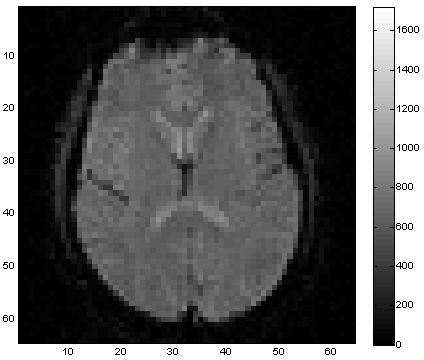
\includegraphics[scale=0.5]{images/good_slice.png}
      \label{fig:good_slice}
   }
   \subfigure{
      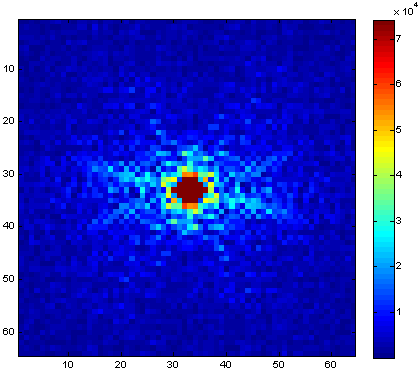
\includegraphics[scale=0.5]{images/good_kspace.png}
      \label{fig:good_kspace}
   }
   \subfigure{
      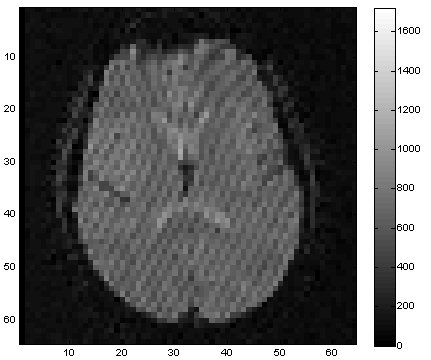
\includegraphics[scale=0.5]{images/spiky_slice.png}
      \label{fig:spiky_slice}
   }
   \subfigure{
      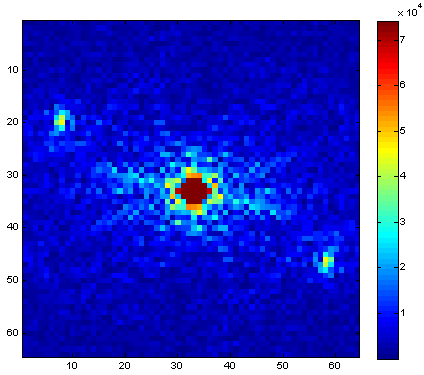
\includegraphics[scale=0.5]{images/spiky_kspace.png}
      \label{fig:spiky_kspace}
   }
  \end{center}
  \caption{Top: A normal EPI slice (left) together with the corresponding reconstruction (by 2D Fast Fourier Transform - fft2) of what the k-space data would have looked like.  One can go back and forth between them by fft2. Bottom: Same, for a "spiky" EPI slice.  Note the spike in k-space, with its symmetric copy, which is the origin of the noise in the image.}
  \label{fig:good_n_spiky_data}
\end{figure}


%%%	%%%	%%%	%%%

\section*{Appendix B: Representative values at 3 mm isotropic voxels}

Following you can find representative indicator values obtained while scanning at 3 mm. isotropic voxels.  Note that the specific values will depend on many things, like where you place your ROIs (especially when using surface coils), reconstruction type (online vs. offline), the length of the run, the bandwidth, the specific task, TR, TE, FA, etc.  As a rule of thumb, the ``raw" \emph{noise}\footnote{this is only true if the electronics noise dominates} should increase with increasing bandwidth as $\sqrt{\mathsf{BW}}$, and the temporal \emph{noise} should decrease with increasing number of volumes as $\sqrt{N}$.

%
\begin{longtable}{cccccl}
\caption{Representative values of data quality indicators for several sessions (separated by horizontal lines).  Included are also the number of volumes and the bandwidth used for each run.  In the notes, 4Ch: 4-channel occipital array}\\
SNR$_0$	& SFNR	& SGR	& Nt		& BW (Hz/Pixel)	& Notes			\\
\hline
\endfirsthead
\caption[]{(continued)}\\
SNR$_0$	& SFNR	& SGR	& Nt		& BW (Hz/Pixel)	& Notes			\\
\hline
\endhead
35.87		& 437.66	& 21.71	& 150	& 4885					& 		\\
36.07		& 378.56	& 22.03	& 150	& 4885					& 		\\
35.94		& 336.28	& 21.59	& 150	& 4885					& 		\\
35.72		& 422.31	& 20.42	& 150	& 4885					& 		\\
35.80		& 360.14	& 20.38	& 150	& 4885					& 		\\
35.64		& 304.14	& 20.98	& 150	& 4885					& 		\\
35.71		& 256.41	& 20.92	& 150	& 4885					& 		\\
35.86		& 389.70	& 20.29	& 150	& 4885					& 		\\
\hline
40.19		& 353.49	& 23.53	& 150	& 4885					& 		\\
39.91		& 356.37	& 23.32	& 150	& 4885					& 		\\
39.80		& 369.80	& 22.87	& 150	& 4885					& 		\\
40.15		& 361.08	& 23.08	& 150	& 4885					& 		\\
39.86		& 352.07	& 22.61	& 150	& 4885					& 		\\
40.25		& 401.14	& 23.02	& 150	& 4885					& 		\\
40.12		& 435.09	& 23.10	& 150	& 4885					& 		\\
39.98		& 304.16	& 23.13	& 150	& 4885					& 		\\
\hline
29.63		& 293.70	& 21.00	& 174	& 4110					& 		\\
32.38		& 250.30	& 17.50	& 174	& 4110					& 		\\
32.52		& 260.01	& 17.92	& 174	& 4110					& 		\\
32.50		& 233.96	& 17.70	& 174	& 4110					& 		\\
32.62		& 226.04	& 17.71	& 174	& 4110					& 		\\
32.52		& 173.57	& 17.78	& 174	& 4110					& 		\\
32.56		& 181.73	& 17.80	& 174	& 4110					& 		\\
32.69		& 173.00	& 17.73	& 174	& 4110					& 		\\
32.77		& 165.65	& 17.65	& 174	& 4110					& 		\\
\hline
29.82		& 178.76	& 18.42	& 192	& 4110					& 		\\
29.62		& 299.35	& 18.68	& 174	& 4110					& 		\\
29.34		& 251.38	& 18.31	& 174	& 4110					& 5 spikes		\\
29.68		& 206.22	& 18.77	& 174	& 4110					& 		\\
29.57		& 226.23	& 18.70	& 174	& 4110					& 		\\
29.75		& 201.03	& 18.86	& 174	& 4110					& 		\\
29.54		& 239.31	& 18.65	& 174	& 4110					& 		\\
29.45		& 241.72	& 18.71	& 192	& 4110					& 1 spike		\\
\hline
33.25		& 512.98	& 24.64	& 60		& 4110					& 		\\
33.38		& 433.44	& 24.10	& 60		& 4110					& 		\\
33.93		& 419.49	& 24.00	& 60		& 4110					& 		\\
32.35		& 392.42	& 24.44	& 60		& 4110					& 		\\
33.74		& 440.53	& 24.11	& 60		& 4110					& 		\\
33.51		& 527.37	& 24.34	& 60		& 4110					& 		\\
34.57		& 493.44	& 24.50	& 60		& 4110					& 		\\
\hline
41.64		& 450.41	& 21.09	& 60		& 4110					& 		\\
41.66		& 670.26	& 21.25	& 60		& 4110					& 		\\
41.68		& 341.18	& 21.08	& 60		& 4110					& 		\\
41.81		& 461.42	& 20.96	& 60		& 4110					& 		\\
41.59		& 364.69	& 20.91	& 60		& 4110					& 		\\
41.58		& 331.81	& 20.64	& 60		& 4110					& 		\\
41.60		& 372.16	& 20.58	& 60		& 4110					& 		\\
\hline
39.78		& 489.56	& 21.81	& 60		& 4110					& 		\\
40.03		& 435.75	& 21.82	& 60		& 4110					& 		\\
40.27		& 411.89	& 21.72	& 60		& 4110					& 1 spike		\\
40.22		& 346.25	& 21.30	& 60		& 4110					& 		\\
40.16		& 366.56	& 21.49	& 60		& 4110					& 		\\
40.52		& 339.34	& 21.14	& 60		& 4110					& 		\\
40.01		& 380.39	& 21.12	& 60		& 4110					& slight motion		\\
\hline
42.69		& 362.61	& 28.31	& 60		& 4110					& 117 spikes	\\
38.93		& 402.02	& 26.09	& 60		& 4110					& 121 spikes	\\
29.94		& 173.68	& 18.36	& 60		& 4110					& 282 spikes	\\
26.03		& 139.84	& 16.91	& 60		& 4110					& 254 spikes	\\
15.48		& 40.97		& 10.06	& 31		& 4110					& 122 spikes	\\
\hline
94.49		& 327.81	& 14.63	& 120	& 4110					& 4Ch \\
94.84		& 272.45	& 14.92	& 120	& 4110					& 4Ch \\
95.67		& 259.96	& 15.59	& 120	& 4110					& 4Ch \\
96.57		& 312.41	& 15.66	& 120	& 4110					& 4Ch \\
96.16		& 384.88	& 15.72	& 120	& 4110					& 4Ch \\
95.42		& 263.48	& 15.70	& 120	& 4110					& 4Ch \\
95.63		& 366.65	& 15.85	& 120	& 4110					& 4Ch \\
\hline
64.56		& 250.26	& 17.16	& 120	& 4110					& 4Ch \\
64.14		& 219.03	& 18.95	& 120	& 4110					& 4Ch \\
65.71		& 212.17	& 18.74	& 120	& 4110					& 4Ch \\
66.08		& 166.46	& 18.15	& 120	& 4110					& 4Ch \\
65.22		& 221.77	& 17.69	& 120	& 4110					& 4Ch \\
65.33		& 192.17	& 17.79	& 120	& 4110					& 4Ch \\
65.03		& 209.05	& 18.15	& 120	& 4110					& 4Ch \\
65.30		& 154.13	& 18.64	& 120	& 4110					& 4Ch \\
\hline
66.98		& 302.94	& 22.77	& 120	& 4885					& 4Ch \\
75.80		& 305.17	& 22.94	& 120	& 4885					& 4Ch \\
50.52		& 459.14	& 23.49	& 120	& 4885					& 4Ch, some motion \\
46.60		& 333.99	& 22.29	& 120	& 4885					& 4Ch, some motion \\
39.74		& 254.47	& 22.20	& 120	& 4885					& 4Ch \\
36.99		& 360.12	& 22.40	& 120	& 4885					& 4Ch, some motion \\
29.97		& 419.24	& 22.68	& 120	& 4885					& 4Ch, some motion \\
27.99		& 347.31	& 21.91	& 120	& 4885					& 4Ch \\
28.51		& 357.73	& 20.57	& 120	& 4885					& 4Ch, some motion \\
\hline
38.03		& 280.76	& 16.21	& 320	& 4110					& 4Ch, 1 spike \\
38.01		& 294.41	& 16.38	& 330	& 4110					& 4Ch \\
38.53		& 292.08	& 16.51	& 330	& 4110					& 4Ch, 1 spike \\
39.05		& 264.91	& 16.63	& 330	& 4110					& 4Ch, 1 spike \\
39.11		& 319.56	& 16.67	& 330	& 4110					& 4Ch \\
39.39		& 268.44	& 16.34	& 330	& 4110					& 4Ch \\
39.42		& 281.92	& 16.24	& 330	& 4110					& 4Ch \\
39.64		& 293.26	& 16.30	& 320	& 4110					& 4Ch, 5 spikes \\
\hline
53.52		& 188.92	& 16.20	& 290	& 4110					& 4Ch \\
53.80		& 178.32	& 16.63	& 290	& 4110					& 4Ch \\
53.85		& 181.67	& 16.61	& 290	& 4110					& 4Ch \\
53.86		& 146.83	& 16.32	& 290	& 4110					& 4Ch \\
54.15		& 173.66	& 16.46	& 290	& 4110					& 4Ch \\
54.03		& 172.10	& 16.44	& 290	& 4110					& 4Ch \\
54.31		& 193.44	& 16.32	& 290	& 4110					& 4Ch \\
54.37		& 213.94	& 16.27	& 290	& 4110					& 4Ch, 3 spikes \\
53.31		& 294.21	& 15.34	& 320	& 4110					& 4Ch \\
54.47		& 186.09	& 16.38	& 320	& 4110					& 4Ch, 1 spike \\
\hline
36.01		& 413.11	& 40.92	& 246	& 4110					& multi-echo		\\
29.78		& 336.29	& 13.40	& 128	& 4165					& multi-echo		\\
38.01		& 198.63	& 23.93	& 225	& 4885 					& 1 spike			\\
35.44		& 463.41	& 24.54	& 200	& 4885					& 17	spikes		\\
31.42		& 49.61		& 21.72	& 168	& 4885					& 30	spikes		\\
\end{longtable}
%




%%%%%   Bibliography   %%%%%%%%

\addcontentsline{toc}{section}{References}
\bibliographystyle{plain}
\bibliography{dataQuality}


% % %

\end{document}